\documentclass{article}
\usepackage[utf8]{inputenc}

\usepackage{amsfonts}
\usepackage{amssymb}
\usepackage{amsmath}
\usepackage{amsthm}
\usepackage{enumitem}

\usepackage{bbold}
\usepackage{bm}
\usepackage{graphicx}
\usepackage{color}
\usepackage{hyperref}
\usepackage[margin=2.5cm]{geometry}

\begin{document}


% ==============================================================================

\title{\Large{INFO8006: Project 2 - Report}}
\vspace{1cm}
\author{\small{\bf Romain LAMBERMONT - s190931} \\ \small{\bf Arthur LOUIS - s191230}}

\maketitle

% ==============================================================================

\section{Problem statement}

\begin{enumerate}[label=\alph*.,leftmargin=*]
    \item In this section, we'll discuss the problem as an adverserial search problem and we'll define all elements of the problem
    \begin{itemize}
        \item \underline{Set of states :} A state in Pacman can be described as :
        \begin{equation*}
            s = \{\text{pacmanPos}, \text{ghostPos}, \text{ghostDirection}, \text{foodMatrix}, \text{score}\}
        \end{equation*}
        Where all terms are respectively : the position of Pacman, the position of the ghost, the direction of the ghost, the food matrix (representing food position with boolean values) and the current score.
        \\
        In this case we can define the initial state $s_0$ like this :
        \begin{equation}
            s_0 = \{\text{pacmanPos}_0, \text{ghostPos}_0, \text{ghostDirection}_0, \text{foodMatrix}_0, 0\}
        \end{equation}
        Where all terms with a $0$ index being initial paramaters given by the layout.
        \item \underline{Player function :} The player can easely be determined this way :
        \begin{equation*}
            \text{player}(s) =  \begin{cases}
                                    0 \text{ if Pacman}\\
                                    1 \text{ if Ghost}
                                \end{cases}
        \end{equation*}                       
        \item \underline{Legal actions :} In a specific state $s$, the set pf legal actions is :
        \begin{equation*}
            \text{action}(s) = \{\text{North, East, South, West}\}
        \end{equation*}
        These actions are only available under the condition that we don't hit a wall if we take the action, thus it depends of the layout.
        \item \underline{Transition model :} The transition model can be described as the result of the action taken on the previous state, giving us the new state $s'$:
        \begin{equation*}
            s' = \text{result}(s,a) = \{\text{pacmanPos} + a, \text{ghostPos'}, \text{ghostDirection'}, \text{foodMatrix'}, \text{score'}\}
        \end{equation*}
        Where all parameters with ' are computed as a response from the action taken $a$ (the ghost reacts at the action taken by Pacman and by taking consideration of its behaviour and the food and score are also updated as a result from the action $a$).
        \item \underline{Terminal test :} The test to check if the state is terminal is simple :
        \begin{equation*}
            \text{terminal}(s) = \begin{cases}
                                    \text{1 if ghost eats Pacman OR Pacman has eaten all dots in foodMatrix}\\
                                    \text{0 Otherwise}
                                 \end{cases}
        \end{equation*}
        \item \underline{Utility function} : The utility function of a Pacman is simply given by the score :
        \begin{equation*} \text{utility}(s,p) = \begin{cases}
                                                    \text{score if }p\text{ = Pacman}\\
                                                    -\text{score if }p\text{ = Ghost}
                                                \end{cases}
        \end{equation*}
        As a reminder the score value is computed using this formula :
        \begin{equation*}
            \text{score} = -\text{time steps} + 10 * \text{eaten dots} - 5 * \text{eaten capsules} + 200 * \text{eaten ghost} + (-500 \text{ if lost}) + (500 \text{ if won})
        \end{equation*}
    \end{itemize}
    \newpage
    \item In the case of a zero-sum game as Pacman the utility function can be described as :
    \begin{equation*}
        \text{utility}(s,p = \text{Ghost}) = \begin{cases}
                                \text{1 if Ghost eats Pacman}\\
                                \text{-1 if Pacman eats all dots}
                              \end{cases}
    \end{equation*}
\end{enumerate}

\section{Implementation}

\begin{enumerate}[label=\alph*.,leftmargin=*]
    \item For an algorithm to be complete, it has to find a solution if one exists. In minimax, we run through all the nodes to find a solution. This only applies if the game tree is finite, so we have to avoid repetition of moves resulting in looping on the same states.
    \\\\
    To avoid this, we keep track of the previously visited nodes and the value of the minimax computation respectively in a set and in a dictionnary (we check if the node is visited thanks to an key function). And by simply looking at the score function we can see 
    that going back on the same states is not useful. Indeed if we find the same node lower in the recursion tree, the score decreases at each time step, so we need to avoid already computed nodes.
    \\\\
    In conclusion, to make the algorithm complete, we would need to modify the set of Legal Moves, including a move to avoid already visited nodes.
    \item \textbf{\textit{Refer to minimax.py .}}
    \item \textbf{\textit{Refer to hminimax(0/1/2).py .}}
    \\\\\underline{Evaluation / cut-off functions :}
    \begin{itemize}
        \item Cut-off : In our 3 different implementations, we'll use the same cut-off function. Indeed, we found it quite simple but still really good with a computation time kept low. 
        Our function just checks if the game is finished (lost or won) or if the depth in the recursion tree exceeds 4 (best relation between computation time and score)
        \item HMinimax0 : Our best heuristic simply uses the Manhattan Distance computation but it is used with an $A^*$ algorithm. It uses a set of Manhattan Distance between Pacman and every food dot.
        Our heuristic function simply returns the lowest Manhattan Distance in the set. This function is used in parralel with 2 other functions, distanceToWin and aStar, that  altogether, gives us a good estimation to find the next optimal node.
        \item HMinimax1 : For our second best heuristic, we use again the combination of the 3 functions (heuristic, distanceToWin, aStar). But this time, we add another variable to the Pacman agent (numActions) that keeps track of the number of calls to the function get\_action. We also use
        use another variable distPacGho that computes the distance between Pacman and the ghost. These two variable are used in a condition that simplifies the computation of the heuristic if Pacman has already moved a lot or if the ghost is far away. The heuristic function used first or when the ghost is far away is :
        \begin{equation*}
            \text{heuristic} = \text{score} - \text{dots remaining} - \text{distance left} - 0.2 * \text{distance Pacman-Ghost}
        \end{equation*}
        Where distance left is the number of steps to make a path between all the dots (using Manhattan Distance) and also take into account the distance between Pacman and the ghost.
        \item HMinimax2 : Our last heuristic is a lot similar to the HMinimax1's one but the formula used is different :
        \begin{equation*}
            \text{heuristic} = \text{score} - 5 * \text{dots remaining} - \text{distance left}
        \end{equation*}
        So we penalize more the fact that there's a lot of food remaining but don't take into account the distance between Pacman and the ghost.
    \end{itemize}
\end{enumerate}

\newpage
\section{Experiment}

\begin{enumerate}[label=\alph*.,leftmargin=*]
    \item \underline{Graphs :} Tested on a MacBook Pro with Intel i5 processor (used only for this task) and Python 3.9.5
    \begin{figure}[!h]
      \centering
      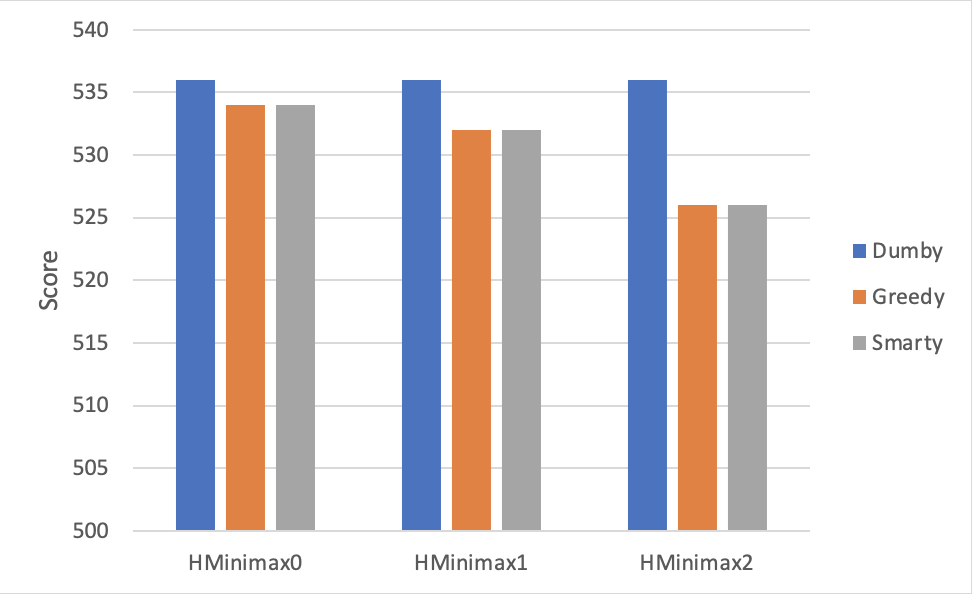
\includegraphics[scale = 0.45]{score.png}
      \caption{Score of different implementations in relation of ghost's type}  
    \end{figure}
    \begin{figure}[!h]
        \centering
        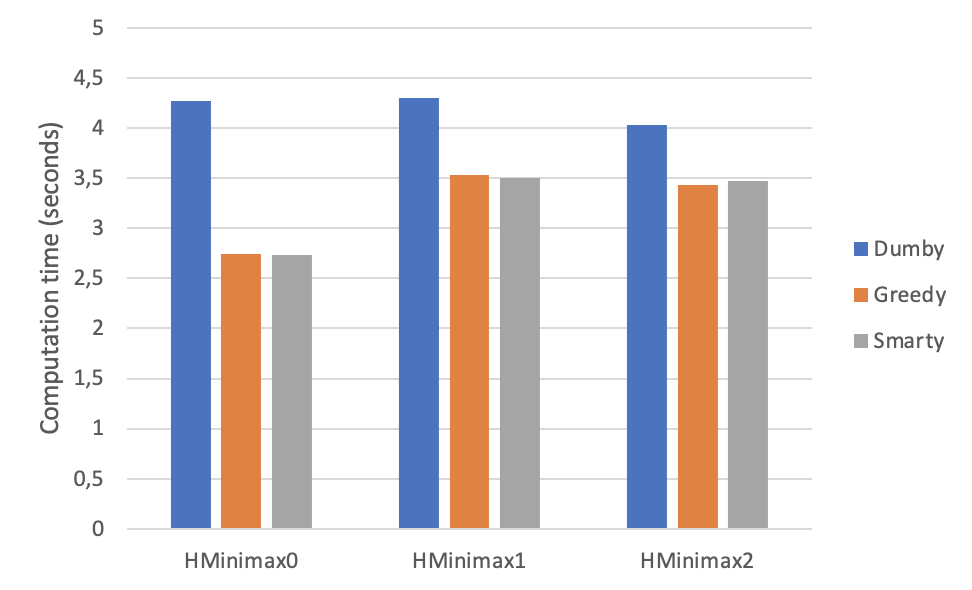
\includegraphics[scale = 0.45]{time.png}
        \caption{Computation time of different implementations in relation of ghost's type}  
    \end{figure}
    \begin{figure}[!h]
        \centering
        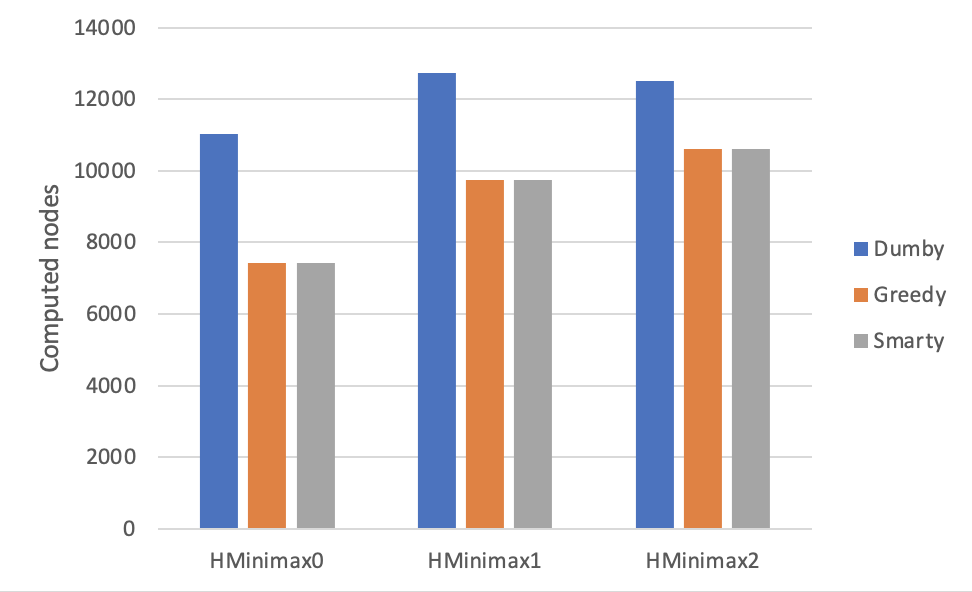
\includegraphics[scale = 0.45]{nodes.png}
        \caption{Computed nodes of different implementations in relation of ghost's type}  
    \end{figure}
    \newpage
    \item As seen on the graphs of previous section, we clearely see that HMinimax0.py is the most efficient one in terms of score, computation time and expanded nodes.
    The two other HMinimax files implement a slightly less efficient method but they're quite similar in terms of performances. This can be explained because the two last files
    look the same with just the heuristic function that differs. Indeed, the cut-off tests and tests in computation to go faster are the same, resulting in similar performances.
    \\\\
    Our first implementation is the best because it is using a combination of "shortest path" (the Manhattan Distance being the fastest way between two positions of the layout without taking care of the walls), and in the case
     of Pacman this method is efficient.
    This provides a good evaluation of the nodes, thus resulting in a good HMinimax.
    \\\\
    For our two last HMinimax, the heuristic evaluation is more classical, it uses a formula that takes multiple parameters and weigh them to get a representation of the game and the nodes we should explore.

\end{enumerate}



% ==============================================================================

\end{document}